\section{Introduction}

\subsection{The iron pnictides}

In 1986 Bednorz and Muller discovered the first high Tc behaviour in a layered cuprate\cite{Bednorz} which started a flurry of research. It later became apparent that the mechanisms of superconuctivity in these materials is more complex than first hoped and some twenty years after the dicovery the exact mechanisms behind the high temperature superconducting behaviour are still not fully understood.

In 2008, the first of a second class of materials that exhibit high-Tc behaviour was discovered by Takahashi et al\cite{Takahashi2008}. Moreover, these materials are generally of a simpler structure than the cuprates and so promise a more direct route to the solution of the high-Tc problem.

These 'iron pnictide' materials are so called becuase they feature one of the pnictogen elements of the periodic table\footnote{The pnictogen elements are N, P, As, Sb, Bi. These are also known as the Group V elements}, typically As or P, in a layer combined with iron. Separating these layers are some rare earth metal, with Eu, K, Ba, Sr and La most commonly employed.

\subsection{Inducing superconductivity}

Superconductivity is not always present in the pnictide materials. One way to induce superconductivity is to apply pressure, another way is to take a relatively simple parent compound and partially substitute one or more elements with another element. In the case of substitution, a series of materials beginning with the simple parent compound and progressing through to the simple end compound --- where substitution is complete --- maps out a phase diagram which features part way along it a region of superconducting phase.

The parent compound \BaFeP through to the end compound \BaFeAs progresses through such a superconducting region\cite{Kasahara2009, Jiang2009} in the series denoted by \BaFePAs and shown in \fig\cite{Figure:PhaseDiagram:Jiang2009}.

\begin{figure}[h]
    \begin{center}
        \includegraphics[scale=0.25]{images/Jiang2009PhaseDiagram}
        \caption{The progression of the \BaFePAs series adapted from reference\cite{Jiang2009}}
        \label{Figure:PhaseDiagram:Jiang2009}
    \end{center}
\end{figure}

The phase diagram shown in \fig\cite{Figure:PhaseDiagram:Jiang2009} is qualitatively similar to many other diagrams of doping, substitutional or pressure progressions in the pnictides which also exhibit a \sdw phase dominating the region over the parent compound which gradually gives way to a superconducting dome which then gives way to a paramagnetic state\cite{Uemura2009}.

For this particular progression of materials the substitution of As for P is isovalent --- both As and P are 3$^{-}$ --- and so does not change the number of charge carriers in the material. The substitution does however reduce the size of the unit cell, predominantly in the $c$ direction with most of the reduction occuring in the FePn (Pn = pnictide) layers\cite{Jiang2009} with the net effect of reducing the tetragonal bond angle.

\begin{figure}[h]
    \begin{center}
        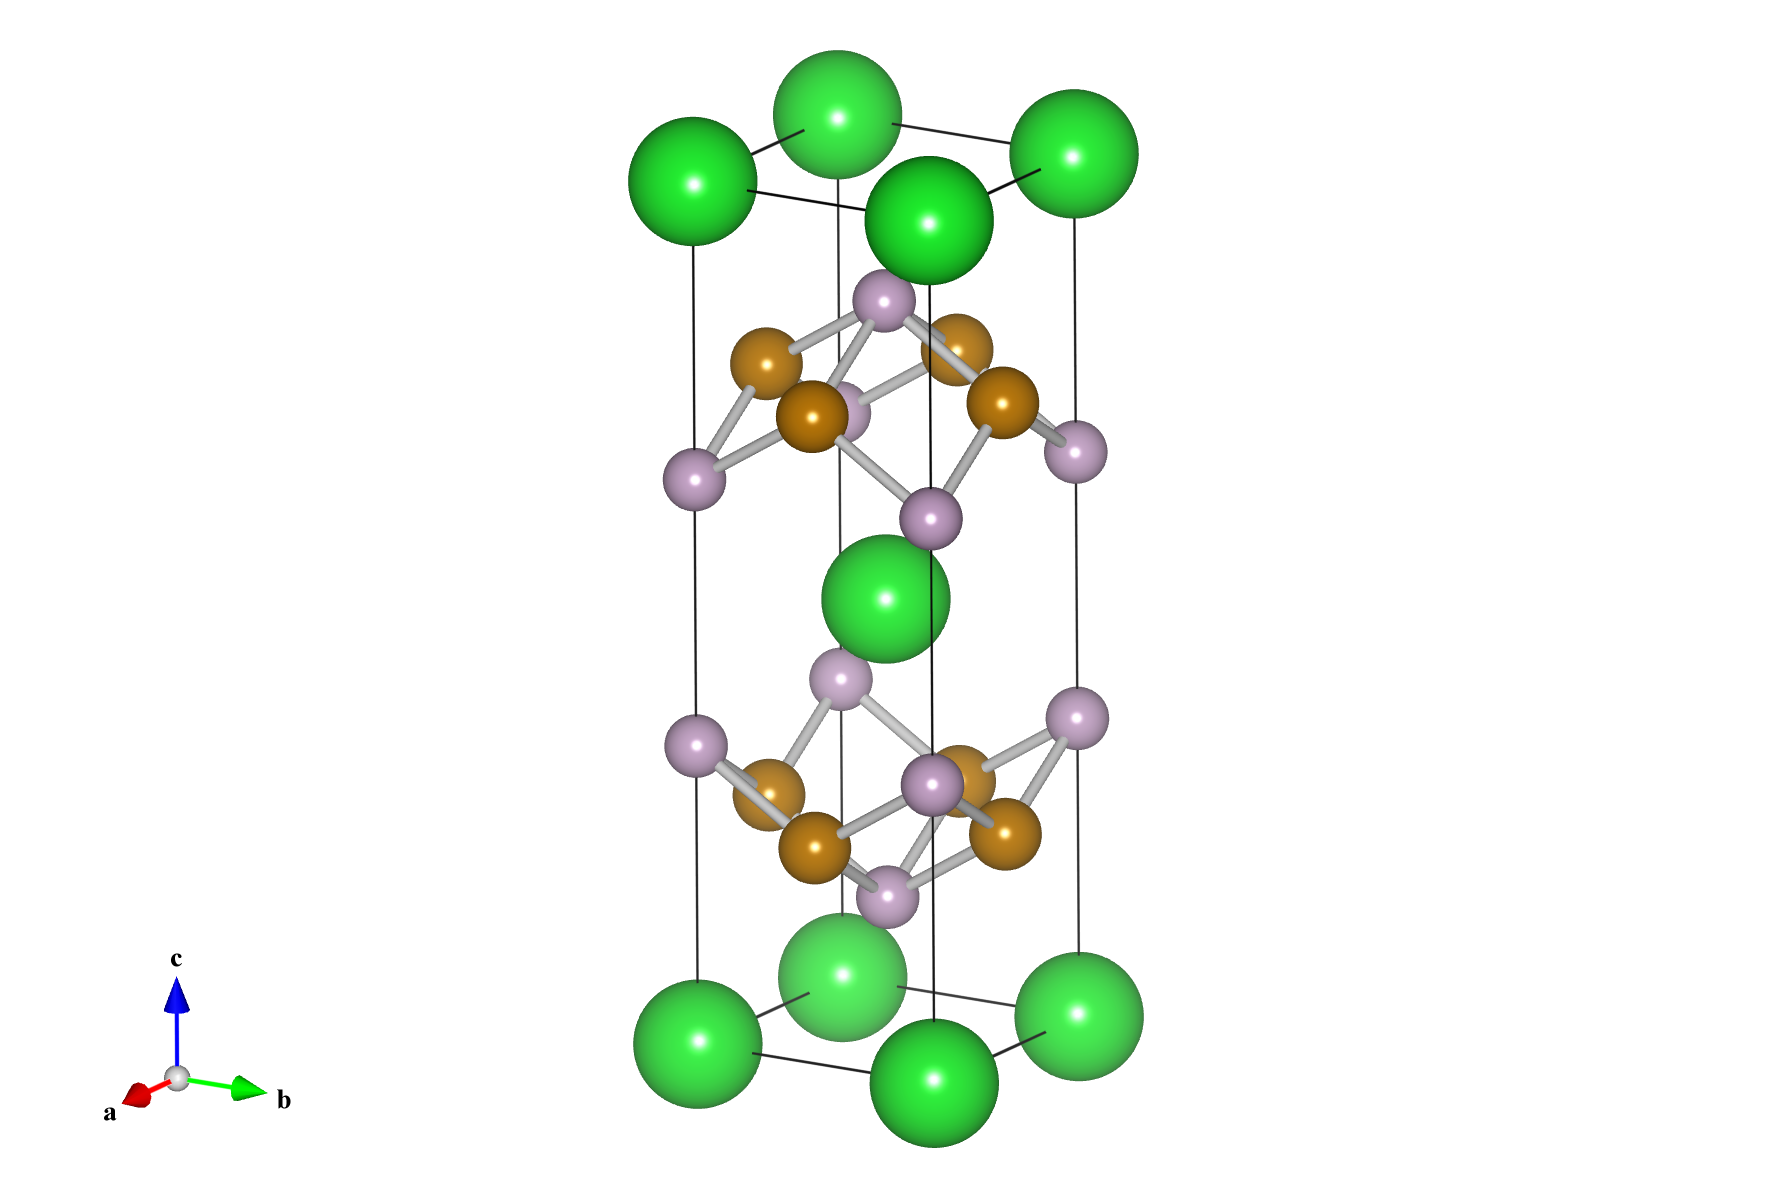
\includegraphics[scale=0.25]{images/BaFeAsPUnitCellTetragonalBondAngle}
        \caption{}
        \label{Figure:BaFeAsPUnitCellTetragonalBondAngle}
    \end{center}
\end{figure}

Several papers have discussed the correlation between the ideal tetrahedral bond angle of \deg and the \Tc of the pnictides\cite{Matsumura2010}
